\subsection{Разработка архитектуры программного средства}
\label{sec:design:architecture}

При разработке сложных приложений можно столкнуться с проблемами, которые, вероятно, возникали раньше и уже имеют большое количество решений.
Такие решения называются шаблонами проектирования.
Они упрощают разработку приложений, поэтому целесообразно их использовать, если есть такая возможность.

Архитектура приложения должна быть приоритетной задачей с самого начала разработки.
Она определяет, как разные элементы программного средства будут соотноситься друг с другом.

Для мобильных приложений характерна проблема постоянно меняющихся подходов и рекомендаций в отображении пользовательского интерфейса.
Для адаптации к таким условиям был придуман шаблон Model-View-ViewModel (т.е. MVVM) -- это шаблон архитектуры клиентских приложений, который был предложен Джоном Госсманом как альтернатива шаблонам MVC и MVP при использовании технологии связывания данных (Data Binding)~\cite{microsoft_mvvm}.
Его концепция заключается в отделении логики представления данных от бизнес-логики путем вынесения её в отдельный класс для более четкого разграничения.

Шаблон состоит из трёх основных компонентов:
\begin{itemize}
    \item Model -- это логика, которая связана с предметной областью и данными, а именно работа с API, базой данных и прочим.
    \item View -- логика, связанная с отображением информации непосредственно пользователю.
    \item ViewModel -- объект, в котором описывается логика поведения View в зависимости от результата работы Model.
    Можно назвать его моделью поведения View.
    Это может быть как форматирование текста, так и логика управления видимостью компонентов или отображения состояний, таких как загрузка, ошибка, пустые экраны и так далее.
    Также в ней описывается поведение, которое было инициировано пользователем (ввод текста, нажатие на кнопку и так далее).
\end{itemize}

Схематичное изображение отношений компонентов шаблона MVVM изображено на рисунке~\ref{fig:design:architecture:mvvm}.
Среди преимуществ данного подхода можно выделить следующие~\cite{android_mvvm}:

\begin{itemize}
    \item Гибкость разработки.
    Этот подход повышает удобство работы в команде, так как пока один член команды работает над компоновкой и стилизацией экрана, другой в это время описывает логику получения данных и их обработки.
    \item Тестирование.
    Такая структура упрощает написание тестов и процесс создания Mock-объектов.
    Также в большинстве случаев отпадает потребность в автоматизированном UI-тестировании, так как можно использовать Unit-тестирование для классов ViewModel.
    \item Разграничение логики.
    За счет большего разграничения код становится более гибким и простым в поддержке.
    Каждый модуль отвечает за свою конкретную функцию.
\end{itemize}

Связь между компонентами View и ViewModel происходит за счёт использования поведенческого шаблона проектирования <<Наблюдатель>>.
Реализация данного шаблона позволяет получать экземпляру объекта оповещения от других объектов об изменении их состояния, тем самым наблюдая за ними без прямой связи с этими.

\begin{figure}[H]
    \centering
    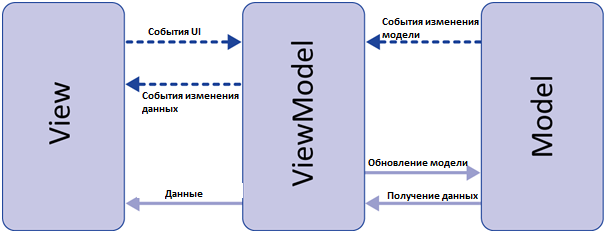
\includegraphics[scale=1]{3_1_mvvm_diagram.png}
    \caption{Схематичное изображение архитектурного шаблона MVVM}
    \label{fig:design:architecture:mvvm}
\end{figure}